\section{问题二：基于变物性闭合的全过程耦合场模型}
\label{sec:p2}

\subsection{相对问题一的增量}

问题二把时间窗从预热段拉长到整个烘干过程，控制方程、坐标与离散格式
全部沿用第~\ref{sec:model}~节，唯一改变的是物性闭合：题面明示经验公式
统一采用附录 3，

\begin{align}
\rho(C)&=650+128C, &
c_p(C)&=1450+2736\,\frac{C}{C+1},
\label{eq:app3_rho_cp}\\
k(C)&=0.21+0.38\,\frac{C}{C+1}, &
D(C,T)&=2.4\times10^{-3}\,\mathrm{e}^{-0.45/C}\,\mathrm{e}^{-3850/T_K},
\label{eq:app3_k_D}
\end{align}

其中 $T_K=T+273.15$ 为热力学温度。式~\eqref{eq:app3_rho_cp}~与~\eqref{eq:app3_k_D}~
在代入时有三处必须辨明的读法。

其一，“统一采用”排除了按阶段切换物性的做法：即使在 $t\le1800$ s 的预热段
也应使用附录 3 而非附录 2。这直接导致问题二在 $1800$ s 处的数值与问题一不同，
后文专门给出对照与解释。

其二，$c_p$ 与 $k$ 中的组合 $C/(C+1)$ 是湿基含水率，不可简化为干基含水率 $C$。
初始状态下该组合等于 $0.7183$，而 $C=2.55$；若误用后者，
热传导系数将由 $0.48296$ 被放大到 $1.179$ W/(m·K)，超过实际值两倍以上。

其三，$D$ 中的 $\mathrm{e}^{-3850/T_K}$ 属于 Arrhenius 型，指数上的 $3850$
已含有活化能与气体常数之比（这与热风干燥中有效扩散系数随温度
呈指数增长的实测规律一致\upcite{singh2018potato}），因此温度必须用热力学温标。
若误用摄氏温标，在 $T=28$ °C 处 $\mathrm{e}^{-3850/28}$ 与
$\mathrm{e}^{-3850/301.15}$ 相差数十个数量级，扩散系数将完全失去意义。
此外 $\mathrm{e}^{-0.45/C}$ 在 $C\to0$ 时需以 $\max(C,10^{-12})$ 保护，
避免烘干末期的除零。

附录 3 只重新给出上述四项，没有重新给出对流换热系数与对流传质系数，
故按假设（5）这两个表面系数沿用附录 2 的 $h=25$ W/(m$^2$·K)、
$h_m=8\times10^{-7}$ m/s。这是不引入任何自由参数的唯一读法。

\subsection{变物性的实际变化幅度}

在 $50$ °C 下 $D$ 随 $C$ 从 $2.55$ 降至 $0.15$ 时由 $1.3471\times10^{-8}$ 降至 $8.0012\times10^{-10}$ m$^2$/s（约 $16.8$ 倍）；而 $28\to50$ °C 使初始 $D$ 提高 $2.39$ 倍。热物性的变化较温和，故变物性的主导影响来自扩散系数；完整轨迹见附录 B。
\iffalse

“变物性”三个字需要量化，否则无法判断它是否真的改变了问题的性质。

\begin{figure}[!htbp]
  \centering
  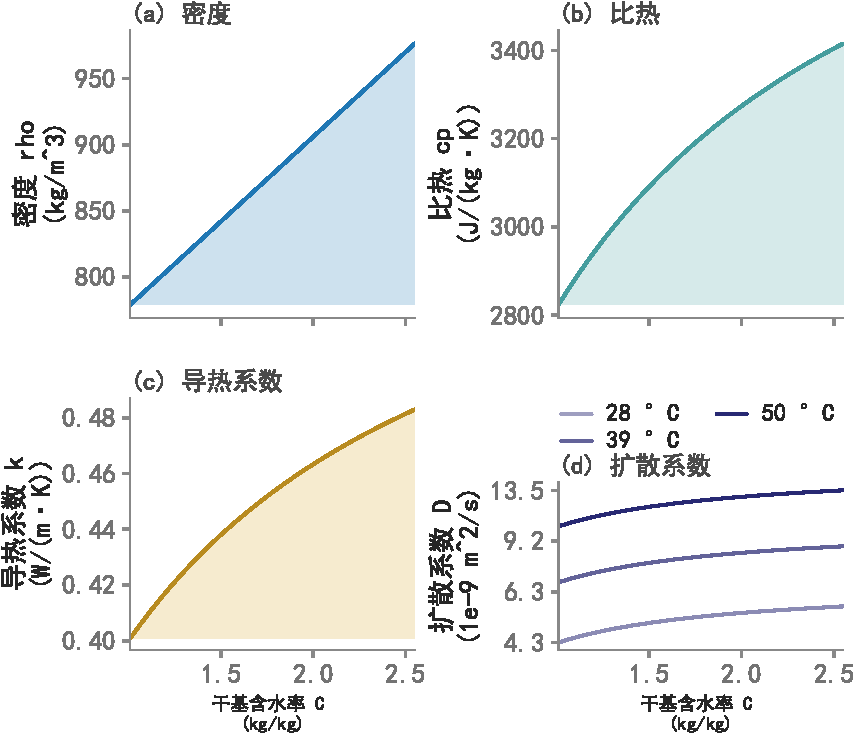
\includegraphics[width=0.8\textwidth,height=0.8\textheight,keepaspectratio]{../figures/fig_q2_props_evolution.pdf}
  \caption{附录三物性随含水率变化}
  \label{fig:q2_props_evolution}
\end{figure}

四项物性沿实际求解轨迹的变化幅度差别悬殊：三项热物性都是温和的单调下降，
只有扩散系数跨越一个数量级（图~\ref{fig:q2_props_evolution}）。
含水率由 $2.55$ 降到阈值 $0.15$ 的过程中，密度由 $976.4$ 降到 $669.2$ kg/m$^3$、
比热容由 $3415.3$ 降到 $1806.9$ J/(kg·K)、热传导系数由 $0.48296$ 降到
$0.25957$ W/(m·K)，三者都是不足一倍的温和变化，且方向一致地下降，
其对热扩散率 $\alpha=k/(\rho c_p)$ 的净影响被大幅抵消——
$\alpha$ 仅由 $1.4483\times10^{-7}$ 升到 $2.1467\times10^{-7}$ m$^2$/s。

扩散系数则完全不同。在 $50$ °C 的平台温度下，$D$ 由 $C=2.55$ 时的
$1.3471\times10^{-8}$ m$^2$/s 降到 $C=0.15$ 时的 $8.0012\times10^{-10}$ m$^2$/s，
降幅 $16.8$ 倍。这一强非线性是全局性的：干燥越接近完成，
水分越难迁移，烘干时长因此不与失水量成正比，而是在末段显著拖长。
本题所谓“变物性”的实质就集中在这一项上。

值得一并指出的是温度对 $D$ 的放大作用。同一含水率 $C=2.55$ 下，
$D$ 由 $28$ °C 时的 $5.6417\times10^{-9}$ 升到 $50$ °C 时的
$1.3471\times10^{-8}$ m$^2$/s，升高 $2.39$ 倍。
这说明热、质两个方程的耦合并非形式上的：预热把药材加热到平台温度，
其真正意义是把扩散系数提高一倍多，为后续脱水创造条件。

\fi
\subsection{烘房条件的时间覆盖}

问题二的时间窗超出附件 1 的覆盖范围，故按第~\ref{sec:model}~节的约定，
$t>14400$ s 后取末 $24$ 点平台均值 $T_{\mathrm{air}}=50.0095$ °C、
$W_{\mathrm{air}}=0.049986$ kg/kg 作常数延拓，绝不线性外推。
制表窗口 $3$ h 恰好落在附件 1 覆盖之内，因此表~\ref{tab:q2_T}~与
表~\ref{tab:q2_C}~的数值完全由实测边界驱动，不含延拓段的影响；
延拓的效力要到问题三与问题四才显现。

\subsection{结果与制表}

\begin{figure}[!htbp]
  \centering
  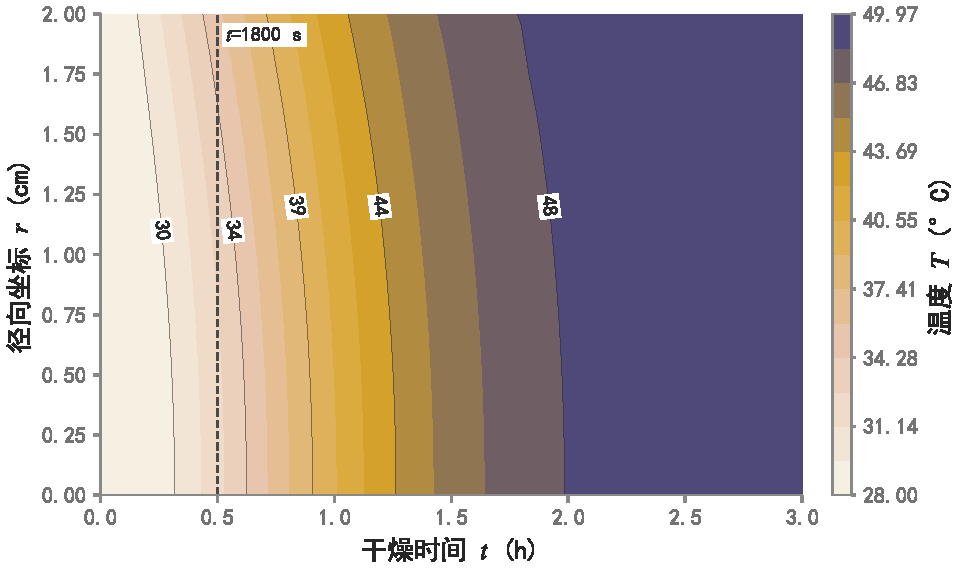
\includegraphics[width=0.74\textwidth,height=0.33\textheight,keepaspectratio]{../figures/fig_q2_field_T.pdf}
  \caption{问题二温度场分布}
  \label{fig:q2_field_T}
\end{figure}

图~\ref{fig:q2_field_T}~中等温线在前 $1$ h 仍明显倾斜，$2$ h 之后几乎垂直，
表明径向温差已被抹平、整根药材随热风同步变化。到 $3$ h 时内外温差
只有 $0.1169$ °C，中心与平台温度的差距为 $0.1600$ °C，
温度场实际上已进入准稳态。

\begin{figure}[!htbp]
  \centering
  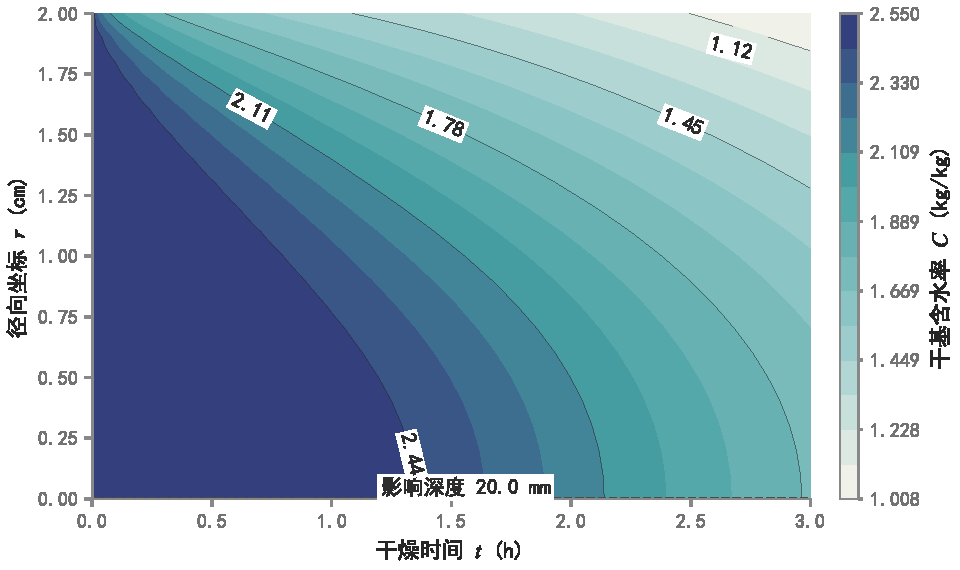
\includegraphics[width=0.74\textwidth,height=0.33\textheight,keepaspectratio]{../figures/fig_q2_field_C.pdf}
  \caption{问题二含水率场分布}
  \label{fig:q2_field_C}
\end{figure}

同一时窗内的含水率场呈现完全不同的形态。图~\ref{fig:q2_field_C}~显示
湿分梯度已从问题一的表皮薄层扩展到整个径向，等值线仍在向中心推进，
没有任何趋于均匀的迹象。到 $3$ h 时中心含水率只完成全程降幅的 $32.7\%$。
两张场图并读给出本题最重要的结构性判断：在这 $3$ h 窗口内热已基本平衡、
质仍在进行。这一判断能外推到后两问的数十小时全程，依据不止于本窗口：
第~\ref{sec:p3}~节的全程解表明温度场此后一直保持准稳态，
而第~\ref{sec:validation}~节的灵敏度排序中热风温度的影响
（$\pm0.5$ °C 对应 $\pm1.6\%$）远小于半径与传质系数。
因此后两问的烘干时长主要由传质控制，温度的作用是通过 Arrhenius 因子
设定扩散系数的水平。需要补充的是，传质本身并非纯内部扩散控制：
$h_m$ 减小 $20\%$ 使时长延长 $2.973\%$，表面对流阻力仍有可测量的份额。

\iffalse
\begin{figure}[!htbp]
  \centering
  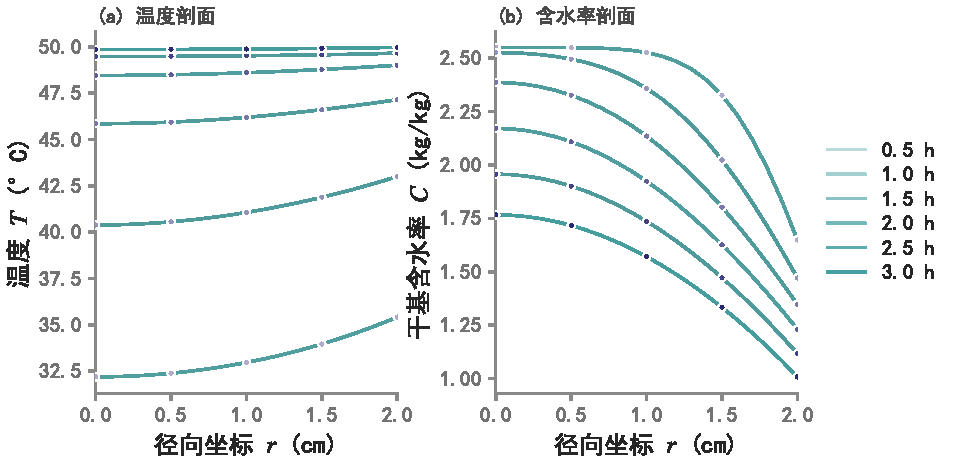
\includegraphics[width=0.9\textwidth,height=0.8\textheight,keepaspectratio]{../figures/fig_q2_profiles.pdf}
  \caption{问题二径向剖面族}
  \label{fig:q2_profiles}
\end{figure}

图~\ref{fig:q2_profiles}~的六条温度剖面逐条压平、间距递减，
与准稳态的判断一致；含水率剖面则保持“中心高、表面低”的单调形状整体下移，
斜率并未变缓。这一单调性是后文把逐点判据化为中心判据的依据。
\fi

\begin{table}[H]
  \centering
  \caption{问题二各时刻各位置温度（°C）}
  \label{tab:q2_T}
  \begin{tabular}{cccccc}
  \toprule
  时刻 (h) & $r=0$ cm & $r=0.5$ cm & $r=1.0$ cm & $r=1.5$ cm & $r=2.0$ cm \\
  \midrule
  0.5 & 32.1900 & 32.3828 & 32.9666 & 33.9614 & 35.4135 \\
  1.0 & 40.3816 & 40.5536 & 41.0605 & 41.8783 & 42.9977 \\
  1.5 & 45.8464 & 45.9345 & 46.1927 & 46.6048 & 47.1398 \\
  2.0 & 48.4500 & 48.4878 & 48.5982 & 48.7733 & 49.0032 \\
  2.5 & 49.4668 & 49.4790 & 49.5135 & 49.5653 & 49.6610 \\
  3.0 & 49.8495 & 49.8553 & 49.8746 & 49.9101 & 49.9664 \\
  \bottomrule
  \end{tabular}
\end{table}

表~\ref{tab:q2_T}~的内外温差由 $0.5$ h 的 $3.2235$ °C 收缩到 $3$ h 的
$0.1169$ °C，一个数量级半的衰减发生在两个半小时内。
与表~\ref{tab:q1_T}~同样需要说明的是：这些温度未计入汽化潜热引起的
表面降温，实际表面温度应略低于表值，第~\ref{sec:validation}~节给出的
$h$ 敏感度约 $0.03\%$ 表明该偏差不会传导为时长的显著变化。

\begin{table}[H]
  \centering
  \caption{问题二各时刻各位置水分浓度（kg/kg）}
  \label{tab:q2_C}
  \begin{tabular}{cccccc}
  \toprule
  时刻 (h) & $r=0$ cm & $r=0.5$ cm & $r=1.0$ cm & $r=1.5$ cm & $r=2.0$ cm \\
  \midrule
  0.5 & 2.5499 & 2.5489 & 2.5255 & 2.3257 & 1.6487 \\
  1.0 & 2.5256 & 2.4948 & 2.3578 & 2.0230 & 1.4711 \\
  1.5 & 2.3860 & 2.3256 & 2.1344 & 1.8020 & 1.3476 \\
  2.0 & 2.1708 & 2.1084 & 1.9236 & 1.6259 & 1.2311 \\
  2.5 & 1.9567 & 1.9006 & 1.7360 & 1.4720 & 1.1167 \\
  3.0 & 1.7662 & 1.7165 & 1.5702 & 1.3333 & 1.0081 \\
  \bottomrule
  \end{tabular}
\end{table}

中心含水率在 $0.5$ h 时几乎未动、$1$ h 后开始明显下降，
到 $3$ h 已降到 $1.7662$ kg/kg（表~\ref{tab:q2_C}）。这个“启动延迟”就是问题一观察到的
湿分渗透过程，只是在更长的时间窗里得以看到它抵达中心之后的行为。
$3$ h 内每隔 $1$ s、每隔 $0.1$ cm 的完整结果见 \verb|result2.xlsx|，
温度与水分浓度各一张工作表，每表 $10800$ 行 $\times$ $22$ 列。

\subsection{与问题一在同一时刻的差异}

问题二在预热段也采用附录 3，故 $1800$ s 的场值与问题一不同；这是物性闭合改变所致而非计算矛盾。完整常/变物性对照见附录 B。
\iffalse

因为问题二在预热段也使用附录 3，两问在 $1800$ s 处必然给出不同数值。
这不是计算不自洽，需要正面交代。

\begin{figure}[!htbp]
  \centering
  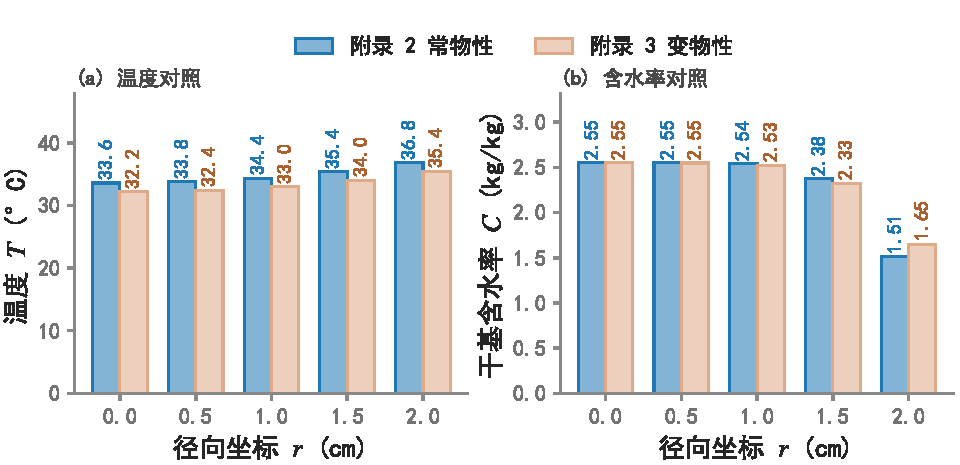
\includegraphics[width=0.9\textwidth,height=0.8\textheight,keepaspectratio]{../figures/fig_q1q2_contrast.pdf}
  \caption{常物性与变物性结果对照}
  \label{fig:q1q2_contrast}
\end{figure}

在 $1800$ s（即本节各表的 $0.5$ h 行）这一共同时刻上并排比较，
两问的温度差与含水率差方向相反
（图~\ref{fig:q1q2_contrast}~给出五个制表半径上的对照）。
温度一侧，问题二整体低于问题一，中心处
$32.1900$ °C 对 $33.5757$ °C，相差 $1.39$ °C。原因可以定量归因：
附录 3 在初始含水率下给出的 $\rho c_p$ 为 $3.335\times10^{6}$ J/(m$^3$·K)，
比附录 2 的 $2.132\times10^{6}$ 大 $56\%$，即同样热流下升温更慢；
热传导系数虽然也更大，但不足以抵消热容的增长，
净结果是热扩散率由 $1.6886\times10^{-7}$ 降到 $1.4483\times10^{-7}$ m$^2$/s。

含水率一侧的差异方向相反且更有意思：问题二的表面含水率 $1.6487$ 反而
高于问题一的 $1.5103$，而内部各点全部低于问题一（$1.0$ cm 处
$2.5255$ 对 $2.5383$）。这是因为附录 3 给出的扩散系数
$5.6417\times10^{-9}$ 比附录 2 的 $4.9377\times10^{-9}$ m$^2$/s 大 $14\%$，
内部水分向表面补充得更快，表面得以维持较高含水率，
而失水被摊到更深的范围。两问的截面平均含水率因此相差不大，
分别为 $2.2936$ 与 $2.2826$ kg/kg。以初始含水率 $C_0=2.55$ kg/kg 为分母折算
累计失水比例 $(C_0-\bar C)/C_0$，两问分别为 $10.06\%$ 与 $10.49\%$，
即问题二多排出 $0.43$ 个百分点。

这组对照说明附录 2 与附录 3 的差别不是简单的“更精确”或“数值更大”，
而是重新分配了热与质的相对快慢。后两问必须在附录 3 及附录 4 各自的
物性闭合下独立计算，不能从问题一的结果外推。
\fi
